\documentclass[10pt, a4paper, onecolumn, oneside, final]{report}

\usepackage[margin=0.37in, bottom=0.58in]{geometry}
\usepackage{tocbibind}
\usepackage{natbib}
\usepackage{subfig}
\usepackage{float}
\usepackage{booktabs}

\usepackage{hyperref}
  \hypersetup{
  	colorlinks=false,
  	pdfborder=0 0 0,
  	linkcolor=blue,
  	citecolor=black,
  	bookmarksopen=false,
  	bookmarksnumbered=true,
  	pdfstartview=FitH,
  	pdfview=FitH
	}
	
\usepackage{url}
  \urlstyle{same}

\usepackage{fancyhdr}

\usepackage{amsmath}
\usepackage{amsfonts}
\usepackage{bm}

\usepackage{listings}
\usepackage{xcolor}
\usepackage{pdfpages}
\usepackage[bahasa]{babel}
\usepackage[fixlanguage]{babelbib}

\definecolor{codegreen}{rgb}{0,0.6,0}
\definecolor{codegray}{rgb}{0.5,0.5,0.5}
\definecolor{codepurple}{rgb}{0.58,0,0.82}
\definecolor{backcolour}{rgb}{0.95,0.95,0.92}

\lstdefinestyle{mystyle}{
    backgroundcolor=\color{backcolour},   
    commentstyle=\color{codegreen},
    keywordstyle=\color{magenta},
    numberstyle=\tiny\color{codegray},
    stringstyle=\color{codepurple},
    basicstyle=\ttfamily\footnotesize,
    breakatwhitespace=false,         
    breaklines=true,                 
    captionpos=b,           
    keepspaces=true,                 
    showspaces=false,                
    showstringspaces=false,
    showtabs=false,                  
    tabsize=2,
    numbers=none
}

\lstset{style=mystyle}

\title{Tugas Kelompok 1\\Aljabar Numerik Kelas A\\Tahun Ajaran 2020/2021}
\author{Eko Julianto Salim, Hocky Yudhiono, Jonathan Nicholas}

\begin{document}
\begin{titlepage}
    \begin{center}\begin{figure}
            \begin{center}
                
\includegraphics[width=2.5cm]{makara.eps}
            \end{center}
        \end{figure}    
        \vspace*{0cm}
        \textbf{
        	UNIVERSITAS INDONESIA\\
        }
        
        \vspace*{1.0cm}
        % judul thesis harus dalam 14pt Times New Roman
        \textbf{Balok Euler-Bernoulli} \\[1.0cm]

        \vspace*{2.5 cm}    
        % harus dalam 14pt Times New Roman
        \textbf{Laporan Tugas Kelompok 1} \\
        
        \vspace*{3 cm}
        \textbf{Kelompok A09} \\
        % penulis dan npm
        
\begin{table}[H]
        \centering
        \begin{tabular}{c c}
            Eko Julianto Salim & 1906350925\\
            Hocky Yudhiono & 1906285604 \\
            Jonathan Nicholas & 1906293133\\
        \end{tabular}
        \end{table}
        \vspace*{5.0cm}

        % informasi mengenai fakultas dan program studi
        \textbf{
        	FAKULTAS ILMU KOMPUTER\\
        	DEPOK \\
        	APRIL 2021
        }
    \end{center}
\end{titlepage}


\section*{Pendahuluan}

Berbagai permasalahan fisika yang ada di sekeliling kita tidak lepas dari perhitungan kontinu dan bilangan-bilangan nyata. Dalam menyusun persamaan dan menyelesaikan permasalahan tersebut, tidak selalu ditemukan metode analisis dalam menghitung secara pasti.

Matematikawan dan ilmuwan komputer sejak dulu sudah meneliti berbagai cara untuk melakukan komputasi dan mengembangkan algoritma yang dapat menyelesaikannya secara cepat. Meskipun solusi yang ditemukan hanya pendekatan dari solusi sesungguhnya, berbagai solusi dengan galat yang lebih kecil masih terus dicari dengan berbagai metode numerik lain. Di era modern ini, ilmu komputer dan informatika berkembang dengan sangat pesat. Salah satu yang menarik ialah permasalahan yang kami angkat pada proyek ini.

\begin{figure}[h]
  \centering
    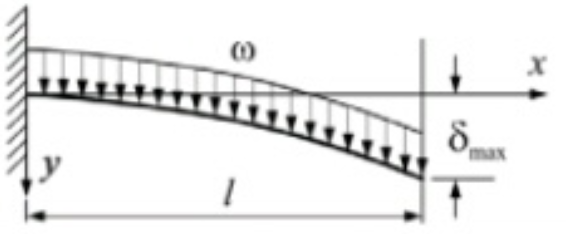
\includegraphics[width=0.3\textwidth]{assets/beam.png}
  \caption{Ilustrasi \textit{cantilever beam}}
\end{figure}

Laporan ini secara umum membahas masalah \textit{vertical displacement} pada sebuah \textit{cantilever beam}, dengan luas momen inersia-nya konstan di sepanjang balok. \textit{Cantilever beam} merupakan struktur sejenis balok dengan satu ujung tetap dan ujung lainnya bebas, layaknya sebuah papan loncat di kolam renang. Teori Balok Euler-Bernoulli menetapkan suatu sistem persamaan matematika yang dapat memodelkan materi ini.

Menariknya, persamaan matematika dalam permasalahan yang terlihat rumit ini ternyata dapat di-reduksi menjadi sebuah sistem persamaan linear, yang dapat dihitung dengan mudah dengan metode numerik. Lebih penting lagi, matriks koefisien yang terbentuk merupakan matriks khusus yang memiliki kompleksitas lebih cepat dibandingkan matriks lain pada umumnya. Dari latar belakang tersebut, kami akan membahas beberapa pertanyaan yang diajukan sebagai pemicu pada proyek ini.

\section*{Isi}

Untuk referensi pertanyaan dari laporan ini mengikuti dokumen \texttt{TK1 Analisis Numerik} yang sudah diberikan.

\subsection*{Soal 1}

Kita sudah mempelajari beberapa algoritma yang bisa digunakan untuk menyelesaikan matriks-matriks \textbf{spesial} yang kompleksitas waktunya lebih cepat. Misalnya pada \textit{banded matrix}, kita bisa melakukan $LU$ \textit{decomposition} yang lebih \textbf{efisien}. Setelah diteliti lebih lanjut, matriks ini membutuhkan \textit{pivoting} agar proses dekomposisi berhasil. Bila tidak, ada entri pada diagonal utama yang bernilai $0$ dalam proses dekomposisi-nya.

Pada dasarnya proses $LU$ \textit{decomposition} sama dengan \textit{Gaussian Elimination}. Pada umumnya $LU$ \textit{decomposition} digunakan karena melakukan \textit{precomputation} terhadap kedua matriks $L$ dan $U$, sehingga saat mencari solusi untuk $b$ lain, tidak perlu melakukan komputasi dengan kompleksitas $O(N^3)$ lagi, melainkan hanya perlu melakukan \textit{forward} dan \textit{backward substitusion} dengan total kompleksitas $O(N^2)$ untuk setiap $b$ yang berbeda.

Cara lainnya ialah menggunakan Eliminasi Gauss. Dengan \textit{bandwidth} yang kecil, pertumbuhan kompleksitasnya terhadap $N$ bisa dibilang sama saat menggunakan dekomposisi $LU$ ataupun eliminasi Gauss. Bila $P$ dan $Q$ yang berturut-turut merupakan lebar pita atas dan bawah dianggap konstan, maka kedua metode tersebut menghasilkan kompleksitas linear.

Demi kemudahan, selain menggunakan \textit{sparse matrix}, kita bisa menggunakan matriks yang disimpan dalam \textit{compact storage}. Digunakan \textit{compact storage} pada dasarnya akan menurunkan kompleksitas memori, dari yang awalnya menyimpan matriks banded dalam kompleksitas memori $O(N^2)$. Kini disimpan dalam $O(N(2Q + P))$. Alasan menggunakannya ialah jelas, karena kemudahan dilakukannya \textit{partial pivoting} saat melakukan Eliminasi Gauss. Dalam kasus ini, kompleksitas memorinya ialah $O(N)$.

\begin{figure}[h]
  \centering
    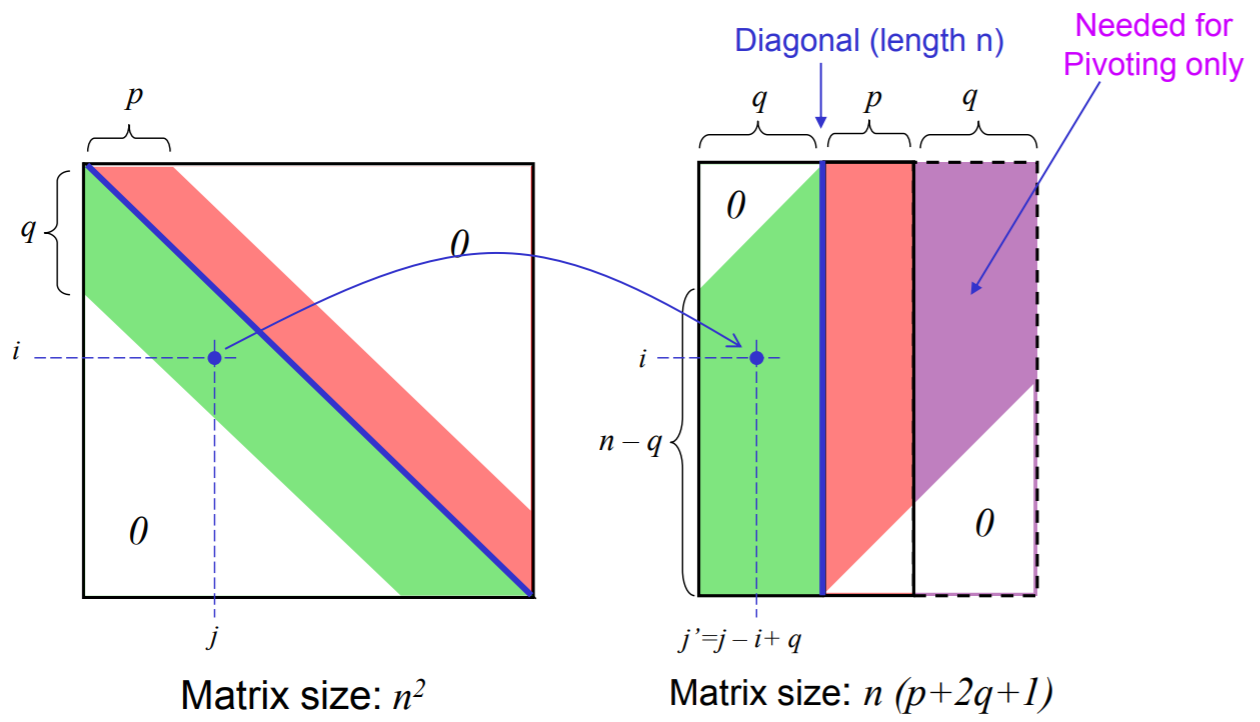
\includegraphics[width=0.3\textwidth]{assets/Compact.png}
  \caption{Ilustrasi \textit{compact storage}}
  \textbf{Source:}  \href{https://ocw.mit.edu/courses/mechanical-engineering/2-29-numerical-fluid-mechanics-spring-2015/lecture-notes-and-references/MIT2_29S15_Lecture7.pdf}{OCW MIT 2.29 Numerical Fluid Mechanics Lecture 7 Slides}
\end{figure}

Disertakan lampiran \texttt{Nomor1/Compact.pdf}. Figur sebelah kiri ialah matriks yang akan direpresentasikan, dan sebelah kanan ialah representasi \textit{compact storage}-nya. Perhatikan bahwa saat dilakukan OBE tukar baris, penyimpanan \textit{floating point} tidak akan melebihi kolom ke-$(P+2Q+1 = 7)$. Selanjutnya, penyelesaian diimplementasikan dengan beberapa alternatif. Ada \texttt{C++} pada lampiran \texttt{Nomor1/Beam.cpp} dan \texttt{Octave} pada \texttt{Nomor1/beamSparse.m} dan \texttt{Nomor1/beamCompact.m}. Ada pula program \texttt{Nomor1/beam.m} yang menghitung nilai $x$ menggunakan fungsi bawaan \texttt{Octave}. Pada program \texttt{C++}, dapat dilakukan pengukuran waktu pada komputasi. Didapatkan waktu pendekatan yang dipaparkan pada tabel berikut.

\begin{table}[ht]
\caption{Hasil Komputasi Program \texttt{Beam.cpp}}
\centering
\begin{tabular}{| c | c | c | c | c |}
\hline
$\bm{n}$ & $10^4$ & $10^5$ & $10^6$ & $10^7$\\
\hline
\textbf{Waktu (s)} & $0.002$ & $0.015$  & $0.289$ & $3.358$\\
\hline
\end{tabular}
\label{table:nonlin}
\end{table}

Terdapat sekitar $2n$ operasi pembagian untuk mencari nilai pembagi setiap iterasi per kolomnya, ada pula operasi $7n$ perkalian dan pengurangan. Untuk substitusi pencarian solusi, akan ada $n$ operasi pembagian, serta $4n$ operasi pengurangan dan perkalian. 

Secara total, ada $3n$ operasi pembagian, $11n$ operasi perkalian, dan $11n$ operasi pengurangan. Perhatikan bahwa operasi pengurangan lebih murah dibandingkan perkalian dan pembagian. Kompleksitas waktu solusi ini ialah $O(n)$. Untuk solusi dari masing-masing $n \in \{10, 20, 40, 80, 100\}$ kami lampirkan pada \texttt{Nomor1/result.txt}.

\subsection*{Soal 2}

Berdasarkan asumsi pada soal, pendekatan turunannya eksak, yang galatnya dekat dengan $\varepsilon_{mach}$, sehingga dapat dicari pendekatan \textit{forward error}-nya menggunakan program yang dilampirkan pada \texttt{Nomor2/yexact.m}. Kemudian di-\textit{plot} dan menghasilkan grafik sebagai berikut.

\begin{table}[H]
\caption{Galat Pendekatan dengan jumlah \textit{steps} berbeda}
\centering
\begin{tabular}{|c|l|l|l|l|l|}
\hline
\textit{\textbf{n}}                       & \multicolumn{1}{c|}{10} & \multicolumn{1}{c|}{20} & \multicolumn{1}{c|}{40} & \multicolumn{1}{c|}{80} & \multicolumn{1}{c|}{100} \\ \hline
\textbf{Absolute Error} & 8.864436e-16 & 6.522560e-15 & 8.9775409e-14 & 1.910711e-13 & 1.89650378e-13 \\ \hline
\end{tabular}
\end{table}

\begin{figure}[H]
    \centering
    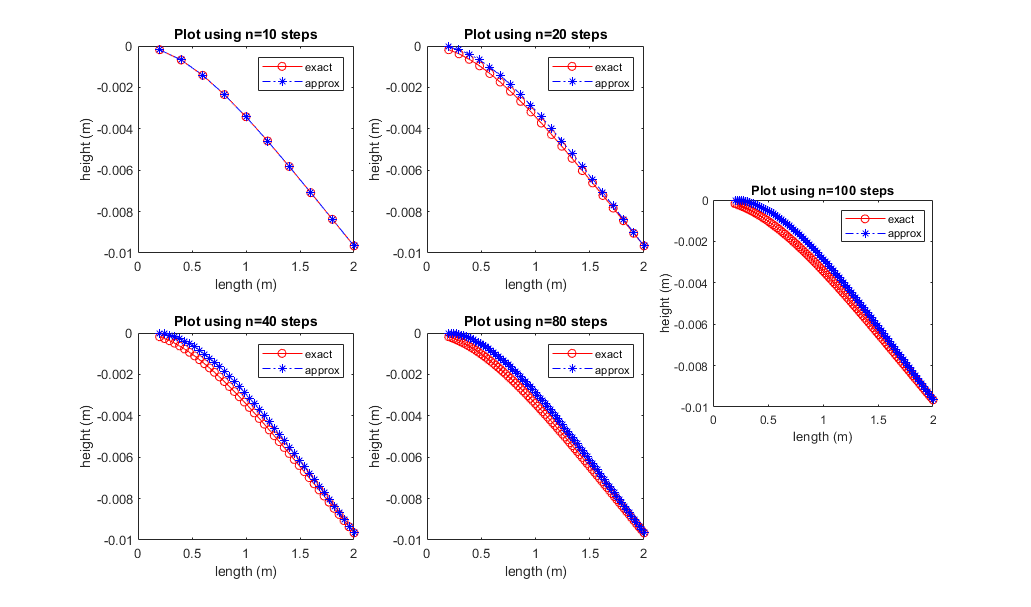
\includegraphics[width=0.7\textwidth]{Nomor2/nomor2.png}
    \caption{Hasil \textit{Plot} untuk $n \in \{10, 20, 40, 80, 100\}$}
    \label{fig:my_label}
\end{figure}

Perlu diobservasi pula, \textit{error}-nya cenderung lebih kecil untuk $x$ yang berada di dekat salah satu ujung dari \textit{beam} tersebut. Untuk $n = 100$, pada ujung $x_n = 2$ meter, \textit{error}-nya sebesar 1.8965e-13 yang nilainya sangat kecil bila dibandingkan $x_{n-1} =$ -1.1708e-05. Hal ini karena pendekatan turunannya pada ujung \textit{beam} seharusnya eksak. Kesalahan tambahan yang mungkin terjadi ialah karena adanya \textit{loss of significance} selama proses eliminasi Gauss.

\subsection*{Soal 3}

Setelah menjalankan program \texttt{Nomor3/nomor3.m} dan menganalisis hasilnya pada sebuah tabel, terlihat bahwa \textit{error} terkecil ketika $k = 1$ dengan $n = 20$. Error dan \textit{condition number} terbesar muncul pada $k$ = 11, yaitu sekitar 4.5e-04 dan 6.6e+17 secara berturut-turut. Saat dibuat grafik kenaikan juga terlihat bahwa untuk $k = 11$ terjadi kenaikan galat yang signifikan. Terlihat bahwa grafik kenaikan \textit{error} proporsional dengan kenaikan yang terjadi pada \textit{condition number}, hanya pada skala yang berbeda yaitu 1e-5 untuk \textit{error} dan 1e16 untuk \textit{condition number}.

\begin{table}[ht]
\caption{Hasil Komputasi \textit{Error} dan \textit{Condition Number}}
\begin{center}
\begin{tabular}{ |c|c|c|c| } 
\hline
$\bm{k}$ & $\bm{n}$ & \textbf{Error} & \textbf{\textit{Condition Number}} \\
\hline
1 & 20 & 6.522560269672795e-15 & 530302.4999985761 \\ 
2 & 40 & 8.977540932875172e-14 & 8449279.999790592 \\ 
3 & 80 & 1.910711172614654e-13 & 134821259.9713538 \\ 
4 & 160 & 2.298145354573400e-11 & 2153877316.211890 \\ 
5 & 320 & 3.551506311261221e-11 & 34434645347.24703 \\ 
6 & 640 & 9.511020391400615e-10 & 550730008901.4839 \\ 
7 & 1280 & 1.916168375706850e-08 & 8809858425614.645 \\ 
8 & 2560 & 2.958674444504539e-07 & 140942219281941.6 \\ 
9 & 5120 & 1.297576218866822e-06 & 2255452034063650 \\ 
10 & 10240 & 2.182653622872545e-05 & 3.645938350988522e+16 \\ 
11 & 20480 & 4.557434849009681e-04 & 6.601799059302159e+17 \\ 
\hline
\end{tabular}
\end{center}
\end{table}

\begin{figure}[h]
    \centering
    \subfloat[\centering error]
        {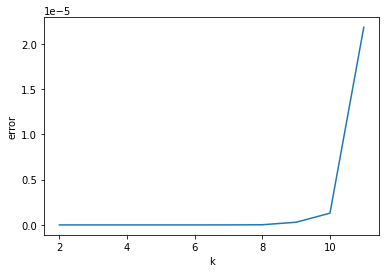
\includegraphics[width=0.3\textwidth]{assets/error.png}}
    \qquad
    \subfloat[\centering condition number]
        {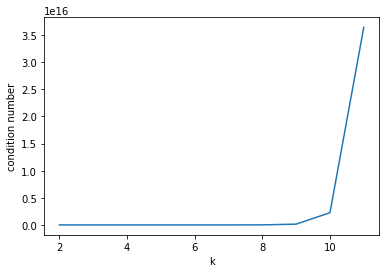
\includegraphics[width=0.3\textwidth]{assets/conditionNumber.png}}
    \caption{\textit{Line plot} $k$ dengan \textit{error} dan \textit{condition number}-nya}
\end{figure}

\textit{Condition number} menyatakan rasio dari nilai terbesar ke nilai terkecil dari sebuah dekomposisi matriks dan merupakan estimasi \textit{worst-case precision loss}.\\ \\

Untuk menganalisis hubungan linear antara \textit{error} dengan \textit{condition number}, kami melakukan komputasi matriks korelasi dengan metode \textit{Pearson R} dan hasilnya pun mengonfirmasi bahwa hubungan dua variabel tersebut linear dengan positif hampir sempurna (mendekati 1). Kesimpulannya adalah fenomena kenaikan \textit{error} ini terjadi karena korelasi positif hampir sempurna antara \textit{condition number} dengan \textit{error}.

\begin{table}[H]
\caption{Matrix korelasi metode \textit{Pearson R}}
\begin{center}
\begin{tabular}{ |c|c|c|c| } 
\hline
 & \textbf{Error} & \textbf{\textit{Condition Number}} \\
\hline
\textbf{Error} & 1.0 & 0.999973 \\
\textbf{\textit{Condition Number}} & 0.999973 & 1.0 \\
\hline
\end{tabular}
\end{center}
\end{table}

\subsection*{Soal 4}

Notasikan sebuah nilai eksak $u$ yang merupakan hasil komputasi numerik. Definisikan pula \textit{step size} $h$, yaitu perbedaan nilai parameter pendekatannya. Definisikan suatu nilai aproksimasi $\bar{u}_h$, dan \textit{order of accuracy} $p$, dengan suatu nilai $C$ yang tidak bergantung terhadap $h$ sehingga berlaku $|\bar{u}_h - u| \leq Ch^p$.

Semakin besar \textit{order of accuracy}-nya, maka akan semakin cepat galatnya berkurang saat $h$ nya menurun. Kita definisikan sebuah \textit{convergence rate} ialah $h^p$. Terkadang galat memiliki suatu perbandingan dengan $h$. Akan ada koefisien galat $D$ sedemikian sehingga $\bar{u}_h - u = Dh^p + O(h^{p+1})$. 

Secara umum, kita dapat mencari \textit{order of accuracy} dengan beberapa cara. Apabila kita mengetahui nilai $u$-nya, seperti di dalam kasus ini, kita bisa menghitung dengan persamaan sebagai berikut.

$$
\begin{aligned}
\log |\bar{u}_h - u| &= \log|Dh^p(1+O(h))|\\
&= \log|Dh^p| + log|1+O(h)|\\
&= \log|D| + p \log h + O(h)
\end{aligned}
$$

Untuk $h_1, h_2, \dots$, masukkan pada suatu fungsi linear dalam $\log h$, untuk mendapatkan nilai pendekatan dari $p$. Dapat di-\textit{plot} nilai dari galat, yaitu $|\bar{u}_h - u|$ sebagai fungsi $h$ di \texttt{Matlab} atau \texttt{Octave}, kemudian akan ditentukan kemiringan garis yang terlihat dari grafiknya. Untuk mendapatkan pendekatan nilai $p$, Dapat dicari gradien melalui perbandingan $u - \bar{u}_h$ dan $u - \bar{u}_{h/2}$. Dapat dituliskan persamaan sebagai berikut.

$$
\begin{aligned}
\frac{\bar{u}_h - u}{\bar{u}_{h/2} - u} &= \frac{Dh^p + O(h^{p+1})}{D(h/2)^p + O((h/2)^{p+1})}\\
&= \frac{D + O(h)}{2^{-P}D + O(h)} = 2^p + O(h)\\
\iff\log_2(\frac{\bar{u}_h - u}{\bar{u}_{h/2} - u}) &= p + O(h)
\end{aligned}
$$

[\cite{kth}]


\subsubsection*{Eksperimen untuk Fungsi Polinom}
Akan digunakan fungsi $f(x) = x^4 + x^3 - 5x^2 + 3x$. Turunan eksaknya ialah $4x^3 + 3x^2 - 10x + 3$. Berikut adalah \texttt{loglog} plot \textit{error} dari metode-metode pendekatan turunan yang disebutkan di soal.
\begin{figure}[h!]
    \centering
    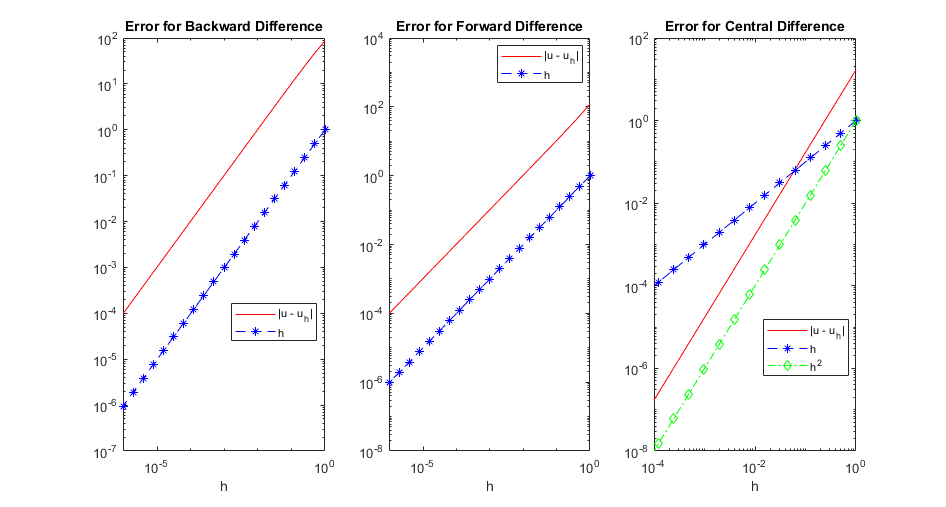
\includegraphics[width=0.5\textwidth]{Nomor4/nomor4-1.png}
    \caption{\textit{Backward, Forward} dan \textit{Central Difference}}
    \label{fig:my_label}
\end{figure}

Perhatikan gambar 5 di atas. Bila di-\textit{plot}, antara $h$, dan menggunakan metode komputasi \textit{Backward Difference}, jelas bahwa garis tersebut terlihat sejajar. Begitu pula untuk \textit{Forward Difference}. Hal ini menunjukkan dengan jelas bahwa \textit{error} mereka proporsional dengan h dan juga bahwa mereka memiliki order akurasi $O(h)$. 

Dalam kasus \textit{Central Difference}, pertumbuhan \textit{error} jauh lebih cepat bila dibandingkan dengan $h$ saja. Bila kita petakan dengan grafik berwarna hijau yang merupakan $h^2$, pertumbuhannya akan terlihat sama. Secara visual, jelas bahwa ini benar dan kita bisa menyimpulkan bahwa metode \textit{Central Difference} memiliki order akurasi $O(h^2)$. Kemudian apabila kita hitung menggunakan pendekatan yang sama dengan yang ada melalui Matlab, didapatkan hasil pada tabel di bawah.

Perhatikan bahwa $\tilde{u}_{h1}$ merepresentasikan pendekatan \textit{Backward Difference}, $\tilde{u}_{h2}$ \textit{Forward Difference} dan $\tilde{u}_{h3}$ \textit{Central Difference}. $a$, $b$, dan $c$ merupakan gradien dari masing-masing pendekatan, di mana pada tahap selanjutnya akan digunakan untuk mencari nilai orde akurasi $p$.

Bisa dilihat bahwa \textit{Central Difference} dengan orde akurasi $O(h^2)$ dapat meminimalisasi \textit{error}-nya dengan \textit{step} yang lebih besar dibandingkan dengan \textit{Backward Difference} dan \textit{Forward Difference} yang memiliki order akurasi $O(h)$. Hal lain yang menarik adalah perbedaan antara \textit{Forward Difference} dan \textit{Backward Difference}, dapat dilihat bahwa \textit{Backward Difference} mendekati nilai dari sisi kiri dan \textit{Forward Difference} mendekati nilai dari sisi kanan.

\begin{table}[H]
\centering
\begin{tabular}{@{}lllllllllll@{}}
\hline
$h$  & $u$   & $\tilde{u}_{h1}$        & $\tilde{u}_{h2}$        & $\tilde{u}_{h3}$        & $a = \frac{\tilde{u}_{h1} - u}{\tilde{u}_{h1/2} - u}$             & $b = \frac{\tilde{u}_{h3} - u}{\tilde{u}_{h3/2} - u}$             & $c = \frac{\tilde{u}_{h3} - u}{\tilde{u}_{h3/2} - u}$ & $p_1 = \log_2{a}$            & $p_2 = \log_2{b}$           & $p_3 = \log_2{c}$           \\ \hline
$2^{0}$                   & 267                    & 180     & 388     & 284     & 1.836                     & 2.166                     & 4  & 0.877                       & 1.115                       & 2    \\
$2^{-1}$                   & 267                    & 219.625 & 322.875 & 271.25  & 1.918                     & 2.083                     & 4  & 0.939                       & 1.058                       & 2    \\
$2^{-2}$                   & 267                    & 242.297 & 293.828 & 268.063 & 1.959                     & 2.041                     & 4  & 0.97 & 1.029                       & 2    \\
$2^{-3}$                   & 267                    & 254.389 & 280.143 & 267.266 & 1.979                     & 2.021                     & 4  & 0.985                       & 1.015                       & 2    \\
$2^{-4}$                   & 267                    & 260.629 & 273.504 & 267.066 & 1.99                      & 2.01                      & 4  & 0.993                       & 1.007                       & 2    \\
$2^{-5}$                   & 267                    & 263.798 & 270.235 & 267.017 & 1.995                     & 2.005                     & 4  & 0.996                       & 1.004                       & 2    \\
$2^{-6}$                   & 267                    & 265.395 & 268.614 & 267.004 & 1.997                     & 2.003                     & 4  & 0.998                       & 1.002                       & 2    \\
$2^{-7}$                   & 267                    & 266.196 & 267.806 & 267.001 & 1.999                     & 2.001                     & 4  & 0.999                       & 1.001                       & 2    \\
$2^{-8}$                   & 267                    & 266.598 & 267.403 & 267     & 1.999                     & 2.001                     & 4  & 1    & 1    & 2    \\
$2^{-9}$                   & 267                    & 266.799 & 267.201 & 267     & 2  & 2  & 4  & 1    & 1    & 2    \\
$2^{-10}$                   & 267                    & 266.899 & 267.101 & 267     & 2  & 2  & 4  & 1    & 1    & 2    \\
$2^{-11}$                   & 267                    & 266.95  & 267.05  & 267     & 2  & 2  & 4  & 1    & 1    & 2    \\
$2^{-12}$                   & 267                    & 266.975 & 267.025 & 267     & 2  & 2  & 4  & 1    & 1    & 2    \\
$2^{-13}$                   & 267                    & 266.987 & 267.013 & 267     & 2  & 2  & 4  & 1    & 1    & 2    \\
$2^{-14}$                   & 267                    & 266.994 & 267.006 & 267     & 2  & 2  & 4.25                      & 1    & 1    & 2.087                       \\
$2^{-15}$                   & 267                    & 266.997 & 267.003 & 267     & 2  & 2  & 4  & 1    & 1    & 2    \\
$2^{-16}$                   & 267                    & 266.998 & 267.002 & 267     & 2  & 2  & -                       & 1    & 1    & -  \\
$2^{-17}$                   & 267                    & 266.999 & 267.001 & 267     & 2  & 2  & -                       & 1    & 1    & -  \\
$2^{-18}$ & 267                    & 267     & 267     & 267     & 2  & 2  & -                       & 1    & 1    & - 
\end{tabular}
\end{table}

\subsubsection*{Eksperimen untuk Pendekatan $y''''$}

Perhatikan persamaan kedua yang terdapat pada dokumen soal, yaitu pendekatan sebagai berikut.

$$
\begin{aligned}
y''''(x) \approx \frac{16y(x-2h)-4y(x-h)+6y(x) - 4y(x+h) + y(x + 2h)}{h^4}
\end{aligned}
$$

Persamaan tersebut menghasilkan \textit{order of accuracy} yang nilainya sangat bervariasi. Hal ini disebabkan karena fungsi $\bar{u}_h - u = Dh^p + O(h^{p+1})$ tidak berlaku, galat yang didapat tidak berbanding lurus dengan nilai $h$. Dalam kasus lain, apabila digunakan persamaan ketiga, yaitu pendekatan sebagai berikut.

$$
\begin{aligned}
y''''(x) \approx \frac{16y(x)-9y(x+h)+\frac{8}{3}y(x+2h) - \frac{1}{4}y(x+3h)}{h^4}
\end{aligned}
$$

Dengan input $x = 2 (\text{meter})$ pada fungsi $y''''(x)$ dan $u = \frac{f}{EI}$, berikut hasil komputasi yang kami peroleh.

% Please add the following required packages to your document preamble:
% \usepackage{booktabs}
\begin{table}[H]
\centering
\begin{tabular}{@{}lllll@{}}
\toprule
$h$ & $\tilde{u}_{h}$ & $u$ & $\frac{\tilde{u}_{h} - u}{\tilde{u}_{h/2} - u}$ & $\log_2{\frac{\tilde{u}_{h} - u}{\tilde{u}_{h/2} - u}}$ \\ \midrule
$2^{0}$                 & -0.0652155384615385    & -0.00482953846153846           & 0.0492686998043481        & -4.34318479018815           \\
$2^{-1}$                 & -1.23047584615385      & -0.00482953846153846           & 0.0571064472803161        & -4.13020255567075           \\
$2^{-2}$                 & -21.4673152307692      & -0.00482953846153846           & 0.059952197430934         & -4.06004355599159           \\
$2^{-3}$                 & -357.998141076923      & -0.00482953846153846           & 0.0612538888370873        & -4.02905475010225           \\
$2^{-4}$                 & -5844.42252015385      & -0.00482953846153846           & 0.061883240807755         & -4.01430743747958           \\
$2^{-5}$                 & -94442.6619096923      & -0.00482953846153846           & 0.0621931436592866        & -4.00710064726394           \\
$2^{-6}$                 & -1518538.08673677      & -0.00482953846153846           & 0.0623469481229747        & -4.00353724777286           \\
$2^{-7}$                 & -24356253.6407257      & -0.00482953846153846           & 0.0624235676821849        & -4.00176537608845           \\
$2^{-8}$                 & -390177212.558594      & -0.00482953846153846           & 0.0624618071966457        & -4.00088187856672           \\
$2^{-9}$                 & -6246652635.67685      & -0.00482953846153846           & 0.0624809094314413        & -4.00044073721222           \\
$2^{-10}$                 & -99976980049.0279      & -0.00482953846153846           & 0.062490456173306         & -4.00022031812493           \\
$2^{-11}$                 & -1599875983810.32      & -0.00482953846153846           & 0.0624952284509642        & -4.00011014644671           \\
$2^{-12}$                 & -25599970165172.3      & -0.00482953846153846           & 0.0624976143165494        & -4.00005507006998           \\
$2^{-13}$                 & -409615158036415       & -0.00482953846153846           & 0.0624988071810402        & -4.00002753424672           \\
$2^{-14}$                 & -6.5539676117319e+15   & -0.00482953846153846           & 0.0624994035962113        & -4.0000137669263            \\
$2^{-15}$                 & -1.04864482452905e+17  & -0.00482953846153846           & 0.0624997017995284        & -4.00000688341389           \\
$2^{-16}$                 & -1.67783972456803e+18  & -0.00482953846153846           & 0.0624998509001199        & -4.00000344169463           \\
$2^{-17}$                 & -2.68454996356608e+19  & -0.00482953846153846           & 0.0624999254501489        & -4.00000172084423           \\
$2^{-18}$                 & -4.29528506511153e+20  & -0.00482953846153846           & 0.0624999627250967        & -4.00000086042135           \\
$2^{-19}$                 & -6.87246020290308e+21  & -0.00482953846153846           & 0.0624999813625539        & -4.00000043021048           \\
$2^{-20}$                 & -1.09959396036246e+23  & -0.00482953846153846           & 0.0624999906812783        & -4.00000021510519           \\
$2^{-21}$                 & -1.75935059889832e+24  & -0.00482953846153846           & 0.0624999953406395        & -4.00000010755258      
\end{tabular}
\end{table}

Dari tabel perhitungan di atas, didapat nilai \textit{order of accuracy} mendekati $-4$. Terlihat bahwa nilai dari pendekatan proporsional terhadap $\frac{1}{h^4}$ (\textit{step size}). Namun, \textit{step size} terlalu kecil dapat menyebabkan sebuah proses membutuhkan waktu yang sangat lama, dan sebaliknya jika \textit{step size} terlalu besar maka hasil yang diperoleh akan konvergen pada suatu nilai yang suboptimal terlalu cepat. 

\section*{Kesimpulan}

Komputasi numerik tidak bisa dihindari dalam beberapa kasus saat menyelesaikan permasalahan matematika, salah satunya ialah dalam kasus \textit{cantilever beam} yang kami analisis melalui laporan ini. Permasalahan matematika yang terlihat kompleks umumnya dapat disederhanakan menjadi permasalahan yang lebih mudah diselesaikan. Berbagai optimisasi juga dapat dilakukan dalam kasus-kasus \textbf{spesial} tertentu. Dalam persoalan ini, matriks \textit{banded} yang entri-entrinya jauh lebih sedikit bisa dimanfaatkan propertinya, misalnya mengganti representasinya dengan \textit{sparse matrix} ataupun \textit{compact storage}.

Dalam komputasi numerik, tidak dapat dihindari akan adanya galat atau \textit{loss of significance} yang diperoleh melalui operasi aritmetika \textit{floating point}. Namun, hal ini dapat diminimalisasi melalui berbagai algoritma yang ada. Lebih baiknya, kita dapat menghitung pendekatan galat melalui rumus yang akan kita gunakan dalam perhitungan. Dalam mencari galat, kita dapat menghitung \textit{backward error} yang merupakan pendekatannya saat dimasukkan ke persamaan awal, maupun mencari \textit{forward error} yang merupakan selisihnya dengan solusi yang paling tepat dengan eksaknya.

Dari analisis yang telah kami lakukan, kami telah mencapai kompetensi lebih dalam bentuk latihan pemrograman dalam \texttt{Matlab} dan \texttt{Octave}. Selain itu, kami juga mempelajari berbagai macam hal, baik dalam memperkuat materi yang sudah dipelajari terutama matriks pita, dekomposisi matriks, dan \textit{backward/forward error}, maupun mempelajari hal baru seperti \textit{step size}, yang merupakan materi yang sangat erat hubungannya dengan \textit{machine learning}.

Alhasil, hal terpenting yang telah kami peroleh dalam pengerjaan analisis ini adalah membangkitkan ketertarikan kami pada dunia matematika yang sangat luas. Kami merasa bahwa materi-materi yang diberikan cukup sulit, namun juga menarik dan berperan sebagai jembatan pembelajaran kami ke topik-topik yang mendatang.

\nocite{*}
\bibliographystyle{apalike}
\bibliography{bibliography.bib}
\pagenumbering{gobble}
\end{document}